
\DeclareRobustCommand{\dlo}[1]{}
\DeclareRobustCommand{\wen}[1]{#1}

\title{Retrieving the leaked signals from noise using a fast dictionary learning method}
\author{Wei Chen\footnotemark[1]\footnotemark[2], Omar M. Saad\footnotemark[3], Yapo Abol{\'e} Serge Innocent Obou{\'e}\footnotemark[4], Liuqing Yang\footnotemark[5], and Yangkang Chen\footnotemark[6]}
\renewcommand{\thefootnote}{\fnsymbol{footnote}}

\address{
\footnotemark[1] Key Laboratory of Exploration Technology for Oil and Gas Resources of Ministry of Education\\
Yangtze University\\
Daxue Road No.111\\
Caidian District\\
Wuhan, China, 430100 \\
\footnotemark[2] Hubei Cooperative Innovation Center of Unconventional Oil and Gas\\
Daxue Road No.111\\
Caidian District\\
Wuhan, China, 430100 \\
\footnotemark[3]
Seismology Department\\
National Research Institute of Astronomy and Geophysics (NRIAG)\\
Helwan 11731, Egypt \\
\footnotemark[4]
School of Earth Sciences\\
Zhejiang University\\
Hangzhou, Zhejiang Province, China, 310027\\
yangkang.chen@zju.edu.cn \\
\footnotemark[5]State Key Laboratory of Petroleum Resources and Prospecting \\
China University of Petroleum \\
Fuxue Road 18th\\
Beijing, China, 102200 \\
\footnotemark[6]Bureau of Economic Geology\\
The University of Texas at Austin\\
University Station, Box X\\
Austin, Texas 78713-8924\\
chenyk2016@gmail.com \\
}

\lefthead{Chen et al.}
\righthead{Retrieving leaked signals}

\begin{abstract}
Most traditional seismic denoising algorithms will cause damages to useful signals, which are visible from the removed noise profiles and are known as signal leakage. The local signal-and-noise orthogonalization method is an effective method for retrieving the leaked signals from the removed noise. Retrieving leaked signals while rejecting the noise is compromised by the smoothing radius parameter in the local orthogonalization method. It is not convenient to adjust the smoothing radius because it is a global parameter while the seismic data is highly variable locally. To retrieve the leaked signals adaptively, we propose a new dictionary learning method. Because of the patch-based nature of the dictionary learning method, it can adapt to the local feature of seismic data. We train a dictionary of atoms that represent the features of the useful signals from the initially denoised data. Based on the learned features, we retrieve the weak leaked signals from the noise via a sparse coding step. Considering the large computational cost when training a dictionary from high-dimensional seismic data, we leverage a fast dictionary updating algorithm, where the singular value decomposition (SVD) is replaced via the algebraic mean to update the dictionary atom. We test the performance of the proposed method on several synthetic and field data examples, and compare it with that from the state-of-the-art local orthogonalization method. 
\end{abstract}

\section{Introduction}
Noise suppression of seismic data plays an important role in seismic exploration \cite[]{abma1995lateral,liuwei2017jge,huang2018damped,omar2020geo1}. In the past decades, numerous methods have been proposed to improve the signal-to-noise ratio (S/N) of seismic data \cite[]{fomel2013seismic,forghani2013effective,han2015microseismic,gomez2016simple,chenwei2018,baimin2018cg,liuwei2019ewt,chenwei2020}. 

The decomposition-based algorithm assumes that the main components of the decomposed seismic data denote the signal while the rest are the noise. Thus, it first decomposes the noisy seismic data into different components through a certain method. Then, the noise components are suppressed by \dlo{shrinkage threshold, truncation, or damping}\wen{shrinking threshold, truncating, or damping} after decomposition. Obviously, the key to decomposition-based methods is whether the decomposition method can effectively decompose the effective signal and noise in the seismic data. The most representative decomposition methods include empirical mode decomposition (EMD) \cite[]{huang1998empirical}, singular value decomposition (SVD) \cite[]{bekara2007local}, and regularized non-stationary decomposition \cite[]{fomel2013seismic,lv2019noise}. Amongst, the denoised method based on the SVD algorithm is also called the rank-reduction-based method. It assumes that the ideal noise-free seismic data is a low-rank matrix, and the random noise will increase the rank of the matrix. Therefore, the random noise attenuation can be regarded as an approximation problem of rank reduction. However, such an assumption is not always true, i.e., the effective signal may exist in the low-rank components, which will cause the damage of the effective signal.

Different from the traditional sparse transform method with analytic basis functions, \wen{dictionary learning (DL) methods adaptively learn the basis functions to best represent the signal features, but at the expense of taking significantly longer computing time \cite[]{aksvd2008,kaplan2009sparse,chen2016double,wujuan2018cg1}}. Instead, it can adaptively obtain a better sparse representation effect according to the characteristics of field seismic data. Therefore, such a method has attracted more and more attention. \cite{kaplan2009sparse} propose a data-driven sparse coding method to adaptively obtain the basis function of sparse representation of seismic data. \cite{beckouche2014simultaneous} divide the seismic data into several small patches, and then use the data in these small patches to train the dictionary, and successfully achieve the signal-and-noise separation of noise corrupted seismic data. By combining the advantages of DL and the traditional sparse transformation method, \cite{chen2016double} propose a double-sparsity dictionary method. It can better represent the signal with specific characteristics in seismic data, and achieve better and more accurate signal-and-noise separation of seismic data. The KSVD-based dictionary learning method obtains the good sparse representation and updated dictionary by iterating and alternately executing the sparse coding and dictionary updating parts \cite[]{abma1995lateral}. The KSVD method obtains successful performance in the sparse-representation-based algorithms, which can not only guarantee the sparse representation to the greatest extent, but also improve the fidelity of the denoising method for seismic data processing \cite[]{sahoo2013dictionary}. However, such a method involves too many SVD operations, which consumes a lot of computational costs. It is not suitable for practical applications in field data, let alone 3-D or even 5-D seismic data. 

In order to improve the computation efficiency of the K-SVD algorithm, \cite{yangkang2020sgk} and \cite{wang2020fast} propose a sequential generalized K-means method (SGK). While maintaining the overall denoising performance, the SGK method greatly improves the computational efficiency. Instead of minimizing the objective function by using the SVD algorithm, SGK exploits the least-squares method to solve the objective function. In the SGK algorithm, the low-rank approximation of the kth dictionary atom by the SVD operation is replaced by a simple summation of training samples. Moreover, based on the special structure of coefficient vectors, \cite{yangkang2020sgk} introduces an accelerated algorithm in the sparse coding procedure of the SGK method. Instead of using orthogonal matching pursuit (OMP) to iteratively get the optimal representation of the target data sample, the sparse coding is implemented for only one time, which greatly enhances the calculation efficiency.

Most traditional methods suffer from the inevitable signal leakage when applied to complex seismic data. The signal leakage refers to those useful signals in the removed noise that appear as spatially coherent.  The signal leakage is caused by either inappropriate parameterization or inappropriate denoising assumptions \cite[]{yangkang2015ortho}. The existence of the signal leakage significantly decreases the quality of the \dlo{denoise}\wen{denoised} seismic data regarding the amplitude fidelity. \cite{yangkang2015ortho} propose an effective way known as the local signal-and-noise orthogonalization method to mitigate the signal leakage in an arbitrary denoising framework. The local orthogonalization method assumes the denoised signal and removed noise to be locally orthogonal to each other and thus compensate for the amplitude loss via solving an inverse problem that is related to the well-known Gram–Schmidt orthogonalization. The local orthogonalization method has been widely used in the seismic community for a variety of different applications, including random noise attenuation \cite[]{yangkang2015ortho}, ground roll noise suppression \cite[]{yangkang2015orthogroll}, multiples elimination \cite[]{zhangdong2020ortho}, elastic wave mode separation \cite[]{sripanich2017elastic}, elastic full-waveform inversion \cite[]{jeong2019enhanced}, etc. However, the local orthogonalization method requires the selection of the smoothing radius parameter, which balances the retrieval of leaked signals and the level of the remaining noise. In addition, due to the inversion nature of the local orthogonalization method, it is highly sensitive to abnormally high amplitude of the erratic noise existing in the data. 

In this paper, we propose to substitute the local orthogonalization method with a new method based on dictionary learning. The new dictionary learning method can obtain equivalent signal retrieval performance but with an easier control on handling small-scale leaked signals due to the patch-based processing. First, we learn the dictionary atoms from the initially denoised data. Then, we code the initial noise section/cube via the learned atoms, where the sparse coefficients corresponding to the leaked signals are high. Next, we apply a percentile thresholding scheme to the sparse coefficients to select those coefficients with distinctly large amplitude. Finally, we reconstruct the extracted leaked signals via the dictionary atoms and the thresholded sparse coefficients. We show that the percentile thresholding plays an important role in distinguishing between noise and leaked signals. Considering the heavy computational cost of the traditional SVD operation, we substitute it with a more efficient SVD-free dictionary learning method. We use different synthetic, 2D, and 3D field data examples to demonstrate the effectiveness of the proposed method, and more importantly, its advantage and flexibility compared with the state-of-the-art local orthogonalization method.

\section{Theory}
\subsection{Retrieving the signal leakage}
Given an arbitrary denoising operator $\mathbf{P}$, the estimation of signal and noise can be expressed as
\begin{align}
\label{eq:sn1}
\mathbf{s} = \mathbf{P}(\mathbf{d}), \\
\label{eq:sn2}
\mathbf{n} = \mathbf{d} - \mathbf{P}(\mathbf{d}),
\end{align}
where $\mathbf{d}$ denotes the input noisy data. However, the estimated signal and noise are not equal to the true signal $\mathbf{s}_{true}$ and true noise $\mathbf{n}_{true}$:
\begin{align}
\label{eq:sn1}
\mathbf{s} \ne \mathbf{s}_{true}, \\
\label{eq:sn2}
\mathbf{n} \ne \mathbf{n}_{true}.
\end{align}
The inaccuracy of the estimated signal is reflected as the signal leakage (spatially coherent signals) in the estimated/removed noise $\mathbf{n}$ and the remaining noise in the estimated signal $\mathbf{s}$. 

The local orthogonalization method can retrieve the leaked signals by
\begin{align}
\label{eq:sn1}
\hat{\mathbf{s}} = \mathbf{s} + \mathbf{w} \circ \mathbf{s}, \\
\label{eq:sn2}
\hat{\mathbf{n}} = \mathbf{n} - \mathbf{w} \circ \mathbf{s}, 
\end{align}
where $\hat{\mathbf{s}}$ and $\hat{\mathbf{n}}$ are the compensated signal and noise after local orthogonalization. $\mathbf{w} \circ \mathbf{s}$ indicates an element-wise product between the weight vector/matrix $\mathbf{w}$ and the initially estimated signal $\mathbf{s}$. 

The local orthogonalization weight $\mathbf{w}$ is solved via iterative inversion and smoothness regularized shaping regularization \cite[]{yangkang2015ortho}. In this paper, we propose a completely different way to retrieve the leaked signals based on dictionary learning\dlo{.}\wen{:} 
\begin{align}
\label{eq:sn1}
\hat{\mathbf{s}} = \mathbf{s} + \mathbf{F}\tilde{\mathbf{M}}, \\
\label{eq:sn2}
\hat{\mathbf{n}} = \mathbf{n} - \mathbf{F}\tilde{\mathbf{M}}, 
\end{align}
where $\mathbf{F}$ denotes a sparse dictionary and $\tilde{\mathbf{M}}$ denotes the optimal representation of the leaked signals (in the form of sparse coefficients) based on the sparse dictionary $\mathbf{F}$. 

The DL method generally achieves the sparse representation of the complex seismic data by alternatively implementing the sparse coding and dictionary update steps. Here, to retrieve the leaked signals, we need to implement the conventional dictionary learning in two steps: (1) first, we obtain the dictionary atoms in $\mathbf{F}$ that follows the structural patterns of the useful signals by learning from the initially denoised data $\mathbf{s}$; (2) second, we use the learned dictionary atoms as the basis functions to code the initially estimated/removed noise $\mathbf{n}$, where the leaked signals will be well represented by the structure-informed atoms as large coefficients. To alleviate the influence of the pure noise in the coefficient matrix, we need to apply a thresholding step. 

\subsection{Sparse coding for retrieving leaked signals}
The initially estimated noise can be divided into $N$ patches $\textbf{n}_{i}$ with $M$ samples (M$\times$1) . Then we can represent the noise in matrix form $\textbf{D}_{n}$ (M$\times$N) with these patches, where \textbf{n}$_{i}$ denotes the data in the $i$th column. We assume the matrix $\textbf{D}_{n}$ can be represented by the multiplication of the dictionary matrix $\mathbf{F}$ and sparse coefficient $\textbf{M}$, which can expressed as:
\begin{equation}
\textbf{D}_{n}=\mathbf{F}\textbf{M}.
\end{equation}
Note that $\textbf{D}_{n}$ has the size of $M\times N$, $\mathbf{F}$ has the size of $M\times L$, and $\textbf{M}$ has the size of $L\times N$. 

Thus, the target of sparse coding is to achieve the dictionary matrix $\mathbf{F}$ and its corresponding sparse coefficient matrix \textbf{M} by solving the following equation:
\wen{\begin{equation}
\label{eq:code}
\hat{\textbf{M}}=\arg\min_{\mathbf{M}}||\textbf{D}_n-\mathbf{F}\textbf{M}||^{2}_{p}, \quad\text{s.t.}  \quad \forall_j ||\textbf{m}_j||_{0}\le Q,
\end{equation}}
where \textbf{M} corresponds to the counterpart of the rearranged data \textbf{D} in the sparse domain, $\mathbf{m}_i$ denotes the $i$th column in \textbf{M}, $||\cdot||_p$ represent $\ell_{p}$ norm of the vector, and $Q$ denotes the sparsity requirement \wen{, e.g., the number of non-zero entries}. Thus, the constraint $\forall_i ||\textbf{m}_i||_{0}\le Q$ indicates that the total number of the non-zero coefficients in each column of \textbf{M} should not exceed Q. Solving inverse problem like equation \ref{eq:code} is an NP-hard problem, which cannot directly obtain the optimal result and is generally solved by the approximation pursuit method. The OMP algorithm is usually exploited to obtain a suitable solution. The pursuit-based method algorithm can be implemented as follows: (1) first, giving an atom and searching the corresponding sparse coefficient of the atoms; (2) then, calculating and decomposing the residual signal by the new given atom; (3) repeating procedure (2) until the requirement is satisfied. 


\subsection{Dictionary learning via KSVD}
To obtain $\mathbf{F}$, a dictionary learning step needs to be implemented. Dictionary learning consists of two separate steps: dictionary update and sparse coding. The sparse coding process is the same as the subsection above, except for substituting the data patches $\textbf{D}_{n}$ created from the initial noise $\mathbf{n}$ with the data patches $\textbf{D}_{s}$ created from the initial signal $\mathbf{s}$. However, the pursuit-based method for sparse coding cannot achieve a satisfactory result at one time. The dictionary should be updated to obtain a good performance. The KSVD method is proposed to better approximate the data features. According to the KSVD algorithm, a matrix of rank K can be recognized as the summation of K matrics of rank 1 as follows:
\begin{equation}
\begin{split}
\mathbf{F}^{i+1}&=\arg\min||\textbf{D}_s-\mathbf{F}\textbf{M}^{i}||^{2}_{p}\\
&=\arg\min||\textbf{D}_{s}-\sum_{j=1}^{L}\textbf{f}_{j}\textbf{m}^{i}_{j}||^{2}_{p}\\
\end{split}\quad,
\end{equation}
where \textbf{f}$_{j}$ and \textbf{m}$_{j}$ are the $j$th column of dictionary matrix $\mathbf{F}$ and sparse coefficient \textbf{M}. \wen{Here, $i$ denotes $i$th iteration.}

One should fix the sparse coefficient \textbf{M} and update the dictionary $\mathbf{F}$ column by column, which can be expressed as follows:
\begin{equation}
\begin{split}
	\mathbf{F}^{i+1}		&=\arg\min||\textbf{D}_{s}-\sum_{j\neq k}^{L}\textbf{f}_{j}\textbf{m}^{i}_{j}-\textbf{f}_{j}\textbf{m}^{i}_{j}||^{2}_{p}\\
	&=\arg\min||\textbf{R}_{k}-\textbf{f}_{k}\textbf{m}^{i}_{k}||^{2}_{p}\\
\end{split}
\quad ,
\end{equation}
where \dlo{\textbf{Q}$_{k}$}\wen{\textbf{R}$_{k}$} denotes the residual between the real data $\textbf{D}_s$ and the sparse representation excluding the $k$th column. Thus, the problem is converted as solving a matrix of rank 1 to approximate \textbf{R}$_{k}$. However, the updated \textbf{m}$_{j}$ will not be sparse if \textbf{R}$_{k}=$\textbf{f}$_{k}$\textbf{m}$_{k}$ is solved directly. To avoid damaging the sparse structure of the coefficient vector \textbf{m}$_{k}$, one should discard the columns in $\textbf{R}_{k}$ where the corresponding element in \textbf{m}$_{k}$ is zero. Here we use $\textbf{R}^{new}_{k}$ and $\textbf{m}_{k}^{new}$ to represent the new residual and the new coefficient vector without non-zero element, and the objective function can be rewritten as:
\begin{equation}
J=||\textbf{R}_{k}-\textbf{f}_{k}\textbf{m}_k||^{2}=||\textbf{R}_{k}^{new}-\textbf{f}_{k}\textbf{m}^{new}_k||^{2}.
\end{equation}
After all the columns of $\mathbf{F}$ are updated, one turns to solve equation \ref{eq:code} for M. Thus, the sparse representation of data is realized when a certain number of iterations is reached. Obviously, there are many SVD operations in the dictionary update step, which is computationally expensive. To overcome such a problem, the SGK-based dictionary update algorithm is proposed. 

\subsection{Dictionary learning via SGK}
The SGK method \cite[]{sahoo2013dictionary,yangkang2020sgk} is also composed of the sparse coding and dictionary update steps. 
 For the first step, there is a slight difference for the constraint compared with the conventional sparse coding. The objective function can be expressed as:
\begin{equation}
\label{eq:sgk1}
\mathbf{F}^{i+1}=\arg\min||\textbf{D}_s-\mathbf{F}\textbf{M}^{i}||^{2}_{p}, \quad\text{s.t.}  \quad \forall_{j}\textbf{m}_{j}=\textbf{e}_{\tau},
\end{equation}
where \wen{\textbf{e}$_{\tau}$ denotes an identity vector}, $\tau$ denotes the \textbf{m}$_{j}$ has all zeros except one in the $\tau$th position. 

The second part, i.e., dictionary updating, is altered as well. Instead of exploiting the SVD, the SGK-based method applies the least-squares method to minimizing the objective function \ref{eq:sgk1}. According to the least-squares method, the gradient of the objective function with respect to the dictionary atoms can be expressed as follows:
\begin{equation}
\label{eq:sgk2}
\frac{\partial J}{\partial \textbf{f}_{k}}=-2(\textbf{R}_{k}^{new}-\textbf{f}_{k}\textbf{m$_{k}^{new}$})(\textbf{m$_{k}^{new}$})^T.
\end{equation}
Thus, the least square solution of the equation \ref{eq:sgk2} can be expressed as follows:
\begin{equation} 
\textbf{f}_{k}=\textbf{R}_{k}^{new}(\textbf{m$_{k}^{new}$})^T(\textbf{m$_{k}^{new}$}(\textbf{m$_{k}^{new}$})^T)^{-1}.
\end{equation}
Using the idea of KSVD-based method for reference, we can rewrite the $\textbf{R}_{k}^{new}$ as follows:
\begin{equation}
\textbf{R}_{k}^{new}=(\textbf{D}_s^{new}-\sum_{j\neq k}^{L}\textbf{f}_{j}\textbf{m$_{j}^{new}$}).
\end{equation}
Since \textbf{m$_{k}^{new}$} (with $N^{k}$ samples) contains ones for all the entries, any column vector multiplied by \textbf{m$_{k}^{new}$} is equal to the summation of all elements of the column vector such as:
\begin{equation}
\begin{split}
\textbf{m$_{k}^{new}$}(\textbf{m$_{k}^{new}$})^T= N^{k},\\
\textbf{D}_s^{new}(\textbf{m$_{k}^{new}$})^T=\sum_{j=1}^{N^{k}}\textbf{d}_{j}.
\end{split}
\end{equation}
Moreover, since $\forall_{j}\textbf{m}_{j}=\textbf{e}_{\tau}$, 
\begin{equation}
\forall_{j\neq k}\textbf{m$_{k}^{new}$}(\textbf{m$_{k}^{new}$})^T=0.
\end{equation}
Thus, we can obtain the updated dictionary atoms as follows:
\begin{equation} 
\textbf{f}_{k}=\frac{1}{N^{k}}\sum_{j=1}^{N^{k}}\textbf{d}_{j}.
\end{equation}
As shown in the derivation of SGK, we can find that the SGK algorithm avoids the time-consuming calculation process. The SVD operation has been replaced by a summation across the training samples.
\subsection{Percentile thresholding of coefficients}
After $\hat{\mathbf{M}}$ is obtained by solving equation \ref{eq:code}, one needs to apply a thresholding step to remove those trivial coefficients that are related to noise:
\begin{equation}
\label{eq:thr}
\tilde{\mathbf{M}} = \mathbf{T} (\hat{\mathbf{M}} ),
\end{equation}
where $\mathbf{T}$ denotes a percentile thresholding operator. The sparse coding model expressed in equation \ref{eq:code} constrains the coefficient matrix $\mathbf{M}$ to be sparse. The sparsity level $Q$ constrains the non-zero entries in each column vector of $\mathbf{M}$. However, due to the fact that not all atoms in the dictionary follow the signal patterns and there are still some atoms contaminated by the noise, a significant portion of the non-zero coefficients in $\mathbf{M}$ correspond to the noise. To suppress the noise, we apply the thresholding to only preserve the largest coefficients that correspond to leaked signals.  The percentile thresholding refers to preserving a certain percentage of largest coefficients rather than preserving the coefficients larger than a certain threshold value. The threshold value varies greatly for different data but the percentage is less dependent on the data, and thus is easier to choose. For example, considering the total number of samples in $\mathbf{M}$ is $L\times N$, the number of non-zero entries is $Q\times N$, then the percentage should be $p\le Q/L$. We will discuss the influence of the percentage later in the Discussion section.

\AtEndDocument{
\begin{figure}[htb!]
\centering
\subfloat[]{\includegraphics[width=0.45\textwidth]{hyper/Fig/hyper}
   \label{fig:hyper}}
   \subfloat[]{\includegraphics[width=0.45\textwidth]{hyper/Fig/hyper-n}
   \label{fig:hyper-n}}
\caption{Synthetic example. (a) Clean data. (b) Noisy data (SNR=1.56 dB).}
\label{fig:hyper,hyper-n}
\end{figure}

\begin{figure}[htb!]
\centering
\subfloat[]{\includegraphics[width=0.3\textwidth]{hyper/Fig/hyper-fx}
   \label{fig:hyper-fx}}
   \subfloat[]{\includegraphics[width=0.3\textwidth]{hyper/Fig/hyper-ortho}
   \label{fig:hyper-ortho}}
   \subfloat[]{\includegraphics[width=0.3\textwidth]{hyper/Fig/hyper-dl}
   \label{fig:hyper-dl}} \\
\subfloat[]{\includegraphics[width=0.3\textwidth]{hyper/Fig/hyper-fx-n}
   \label{fig:hyper-fx-n}}
   \subfloat[]{\includegraphics[width=0.3\textwidth]{hyper/Fig/hyper-ortho-n}
   \label{fig:hyper-ortho-n}}
   \subfloat[]{\includegraphics[width=0.3\textwidth]{hyper/Fig/hyper-dl-n}
   \label{fig:hyper-dl-n}} 
\caption{Synthetic example. Denoised data using (a) FX method (SNR=6.37 dB), (b) local orthogonalization method (SNR=7.78 dB), and (c) proposed method (SNR=9.13 dB). (d)-(f) Removed noise corresponding to (a)-(c).}
\label{fig:hyper-fx,hyper-ortho,hyper-dl,hyper-fx-n,hyper-ortho-n,hyper-dl-n}
\end{figure}

\begin{figure}[htb!]
\centering
\subfloat[]{\includegraphics[width=0.3\textwidth]{hyper/Fig/hyper-fx-s}
   \label{fig:hyper-fx-s}}
   \subfloat[]{\includegraphics[width=0.3\textwidth]{hyper/Fig/hyper-ortho-s}
   \label{fig:hyper-ortho-s}}
   \subfloat[]{\includegraphics[width=0.3\textwidth]{hyper/Fig/hyper-dl-s}
   \label{fig:hyper-dl-s}} 
\caption{Synthetic example. Local similarity between denoised data and removed noise using (a) FX method, (b) local orthogonalization method, and (c) proposed method. }
\label{fig:hyper-fx-s,hyper-ortho-s,hyper-dl-s}
\end{figure}


\begin{figure}[htb!]
\centering
\subfloat[]{\includegraphics[width=\textwidth]{hyper/Fig/hyper-comp}}
\caption{Denoising comparison. From left to right: initial result, initial noise, recovered leaked signals, new result, new noise.}
\label{fig:hyper-comp}
\end{figure}

\begin{figure}[htb!]
\centering
\subfloat[]{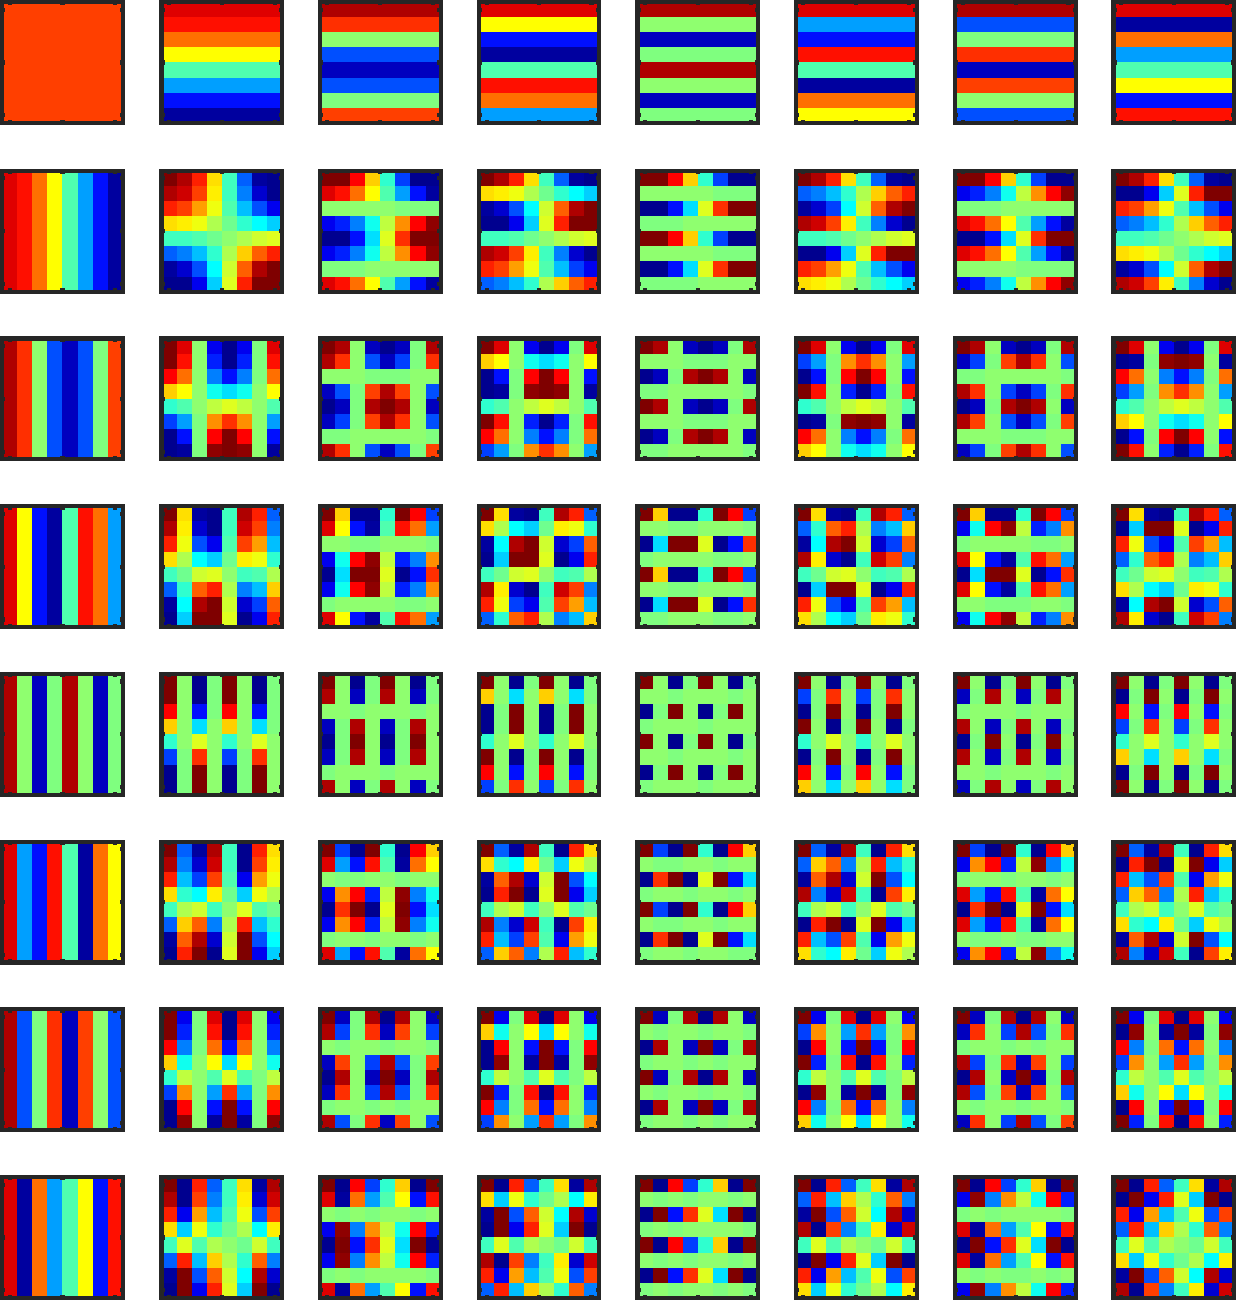
\includegraphics[width=0.5\textwidth]{Fig/atoms1}
   \label{fig:atoms1}}\\
   \subfloat[]{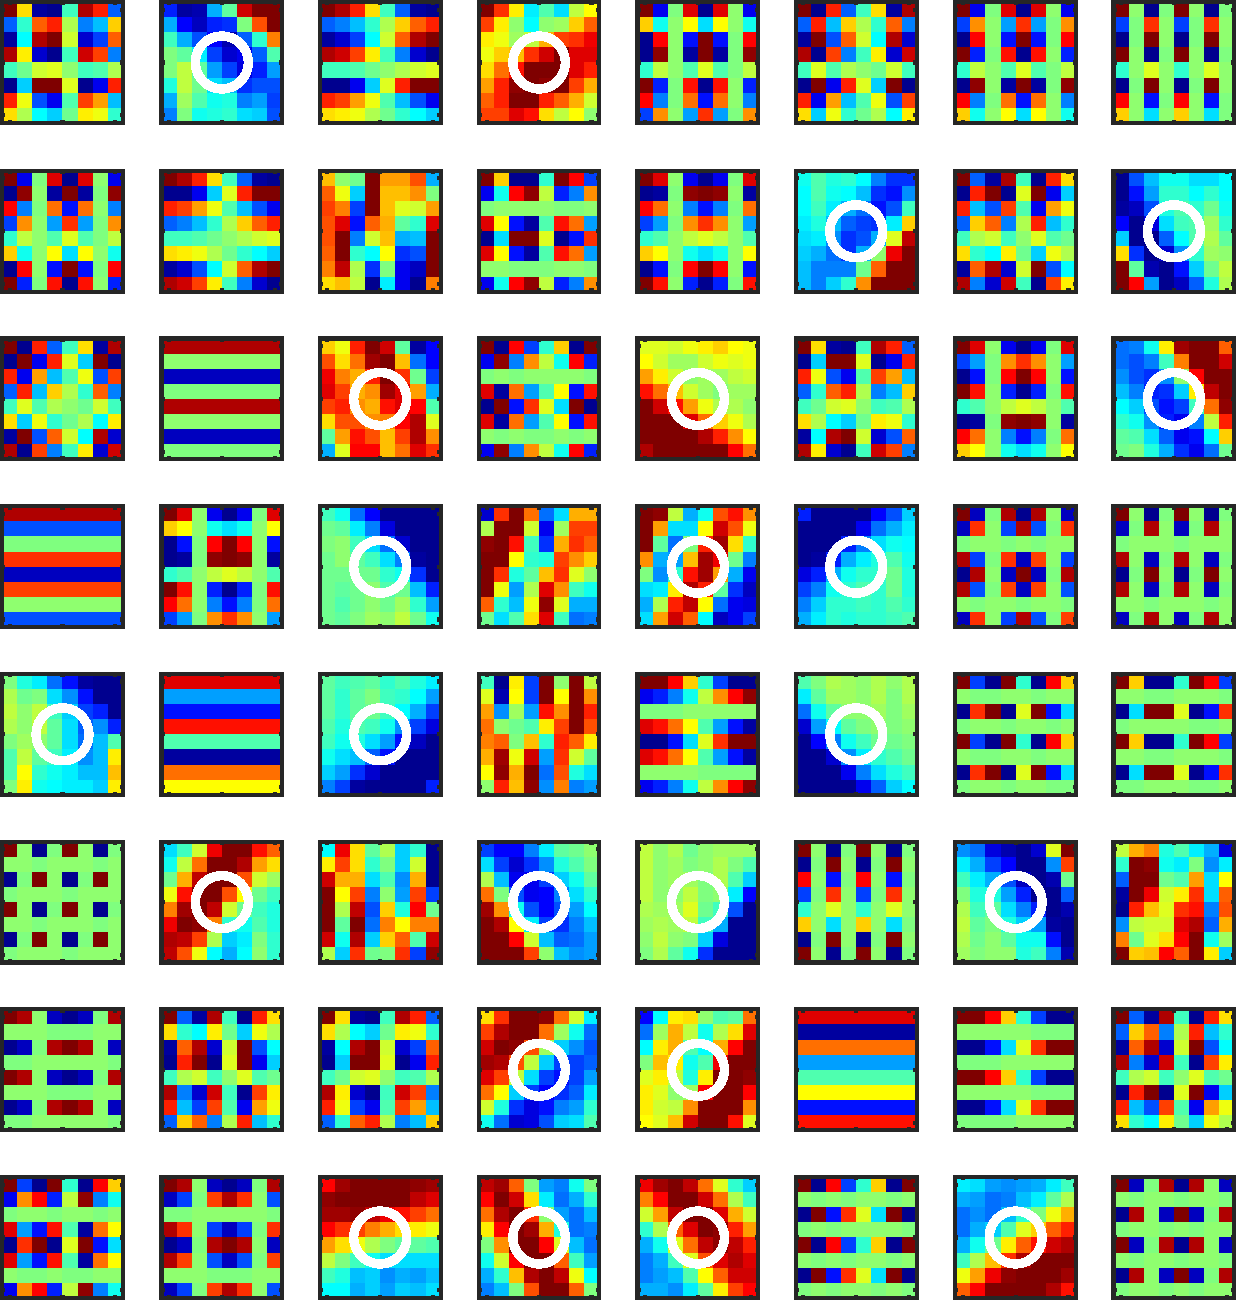
\includegraphics[width=0.5\textwidth]{Fig/atoms2}
   \label{fig:atoms2}}
\caption{Comparison between the initial atoms (a) and learned atoms (b). The white circles in (b) show clear features of the seismic signals learned by the SGK method.}
\label{fig:atoms1,atoms2}
\end{figure}

\begin{figure}[htb!]
\centering
   \subfloat[]{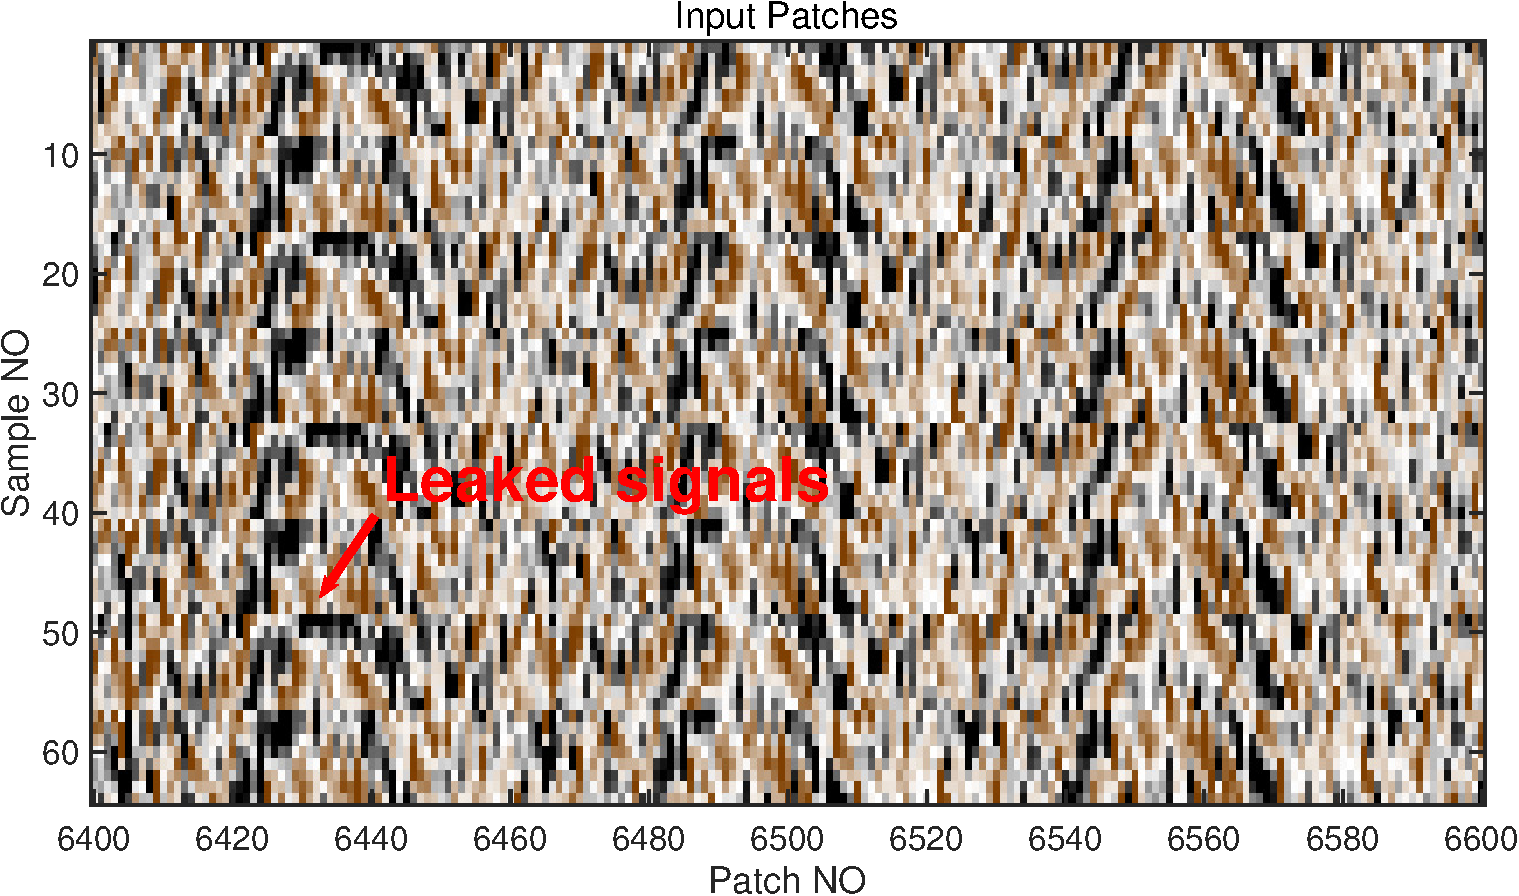
\includegraphics[width=0.7\textwidth]{Fig/hyper_XXn_z}
   \label{fig:hyper_XXn_z}}\\
   \subfloat[]{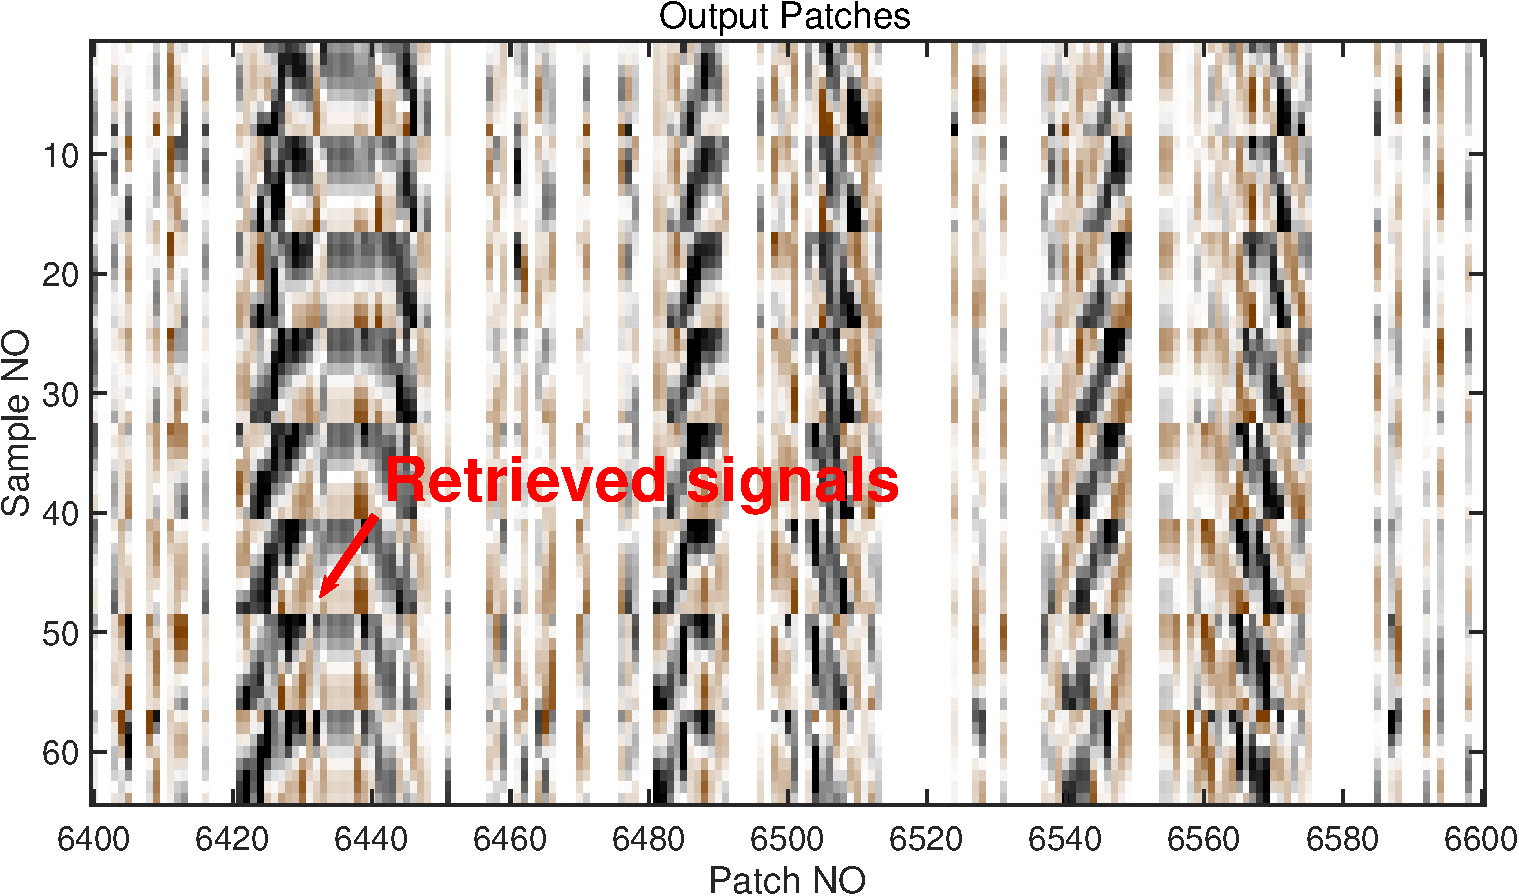
\includegraphics[width=0.7\textwidth]{Fig/hyper_Xn_z}
   \label{fig:hyper_Xn_z}}
\caption{Comparison of different patches. \old{(a) Input patches created from the initial noise. (b) Zoomed patches from (a). (c) Output patches after dictionary learning and thresholding. (d) Zoomed patches from (b). The zooming areas are highlighted by the red frame boxes. Note the clear retrieved signal patches.}\new{(a) Input patches created from the initial noise. (b) Output patches after dictionary learning and thresholding.} }
\label{fig:hyper_XXn_z,hyper_Xn_z}
\end{figure}
}
\section{Examples}
We test the effectiveness of the proposed method using a synthetic dataset, and several 2D and 3D real seismic datasets. We benchmark the proposed method with the state-of-the-art local orthogonalization method, which is proposed specifically for retrieving the leaked signals. For the synthetic data, we quantitatively evaluate the denoising performance using the SNR method:
\begin{equation}
\label{eq:snr}
\text{SNR}=10\log_{10}\frac{\Arrowvert \mathbf{s} \Arrowvert_2^2}{\Arrowvert \mathbf{s} -\hat{\mathbf{s}}\Arrowvert_2^2},
\end{equation}
where $\mathbf{s}$ is the clean data, and $\hat{\mathbf{s}}$ is the noisy or denoised data. 

The first example is a synthetic dataset, as plotted in Figure \ref{fig:hyper,hyper-n}. There are four hyperbolic events in the data. Figures  \ref{fig:hyper} and \ref{fig:hyper-n} show the clean and noisy data, respectively. The noise is additive and bandlimited random noise. Based on the definition in equation \ref{eq:snr}, the SNR of the noisy data is 1.56 dB. Figure \ref{fig:hyper-fx,hyper-ortho,hyper-dl,hyper-fx-n,hyper-ortho-n,hyper-dl-n} plots a comparison of denoised data using three different methods and their corresponding noise sections. Figures \ref{fig:hyper-fx} and \ref{fig:hyper-fx-n} correspond to the FX method. It is clear that significant signal leakage is observable in the removed noise. Figures \ref{fig:hyper-ortho} and \ref{fig:hyper-ortho-n} correspond to the local orthogonalization method. It is obvious that the local orthogonalization method retrieves a significant amount of leaked signal energy but causes a small amount of leaked signals in the noise. Figures \ref{fig:hyper-dl} and \ref{fig:hyper-dl-n} correspond to the proposed method, where almost all the leaked signals have been retrieved and the denoised signals become stronger. \wen{The artifacts in 1.5 s are caused due to the deficiency of the FX method, e.g., the failure of the FX method to accurately estimate the prediction filter at the notch frequencies due to a superposition of several Ricker wavelets at different time positions.} The SNRs of the results from FX, local orthogonalization, and the proposed methods are 6.37 dB, 7.78 dB, and 9.13 dB, respectively. Another metric to evaluate the denoising performance is the local similarity between the denoised data and removed noise. A high local similarity means a higher probability that the signal is leaked. The local similarity metric can effectively detect those areas with strong signal leakage \cite[]{yangkang2015ortho}.  The local similarity comparison is shown in Figure \ref{fig:hyper-fx-s,hyper-ortho-s,hyper-dl-s}. It is clear that the local similarity corresponding to the proposed method is generally the smallest. 

To compare the difference between different data and further demonstrate what the proposed method has retrieved, we plot different data side by side in Figure \ref{fig:hyper-comp}. In Figure \ref{fig:hyper-comp}, from left to right, it corresponds to the initial result, initial noise, recovered leaked signals, new result, new noise. It is clear that the dictionary learning process only retrieves the leaked signals without random noise. We show a comparison of the initial dictionary atoms in Figure \ref{fig:atoms1} and the learned dictionary atoms in Figure \ref{fig:atoms2}. From Figure \ref{fig:atoms2}, it is clear that the fast dictionary learning method can successfully extract some signal features from the initially denoised data. The white circles highlight those obvious signal features extracted from the data. We also show a comparison between the patches generated from the initial noise (Figure \ref{fig:hyper_XXn_z}) and the denoised patches (Figure \ref{fig:hyper_Xn_z}), which correspond to the retrieved leaked signals. \old{To visualize clearly the patches, we zoom in some patches and show them in the right column of Figure \ref{fig:hyper_XXn_z,hyper_Xn_z}.} It is clear that the dictionary learning method successfully retrieves those leaked signals from the noise patches. The zooming areas are highlighted by the red frame boxes in the left column of Figure \ref{fig:hyper_XXn_z,hyper_Xn_z}.
\AtEndDocument{
\begin{figure}[htb!]
\centering
\subfloat[]{\includegraphics[width=0.45\textwidth]{real2d/Fig/pp-0}
   \label{fig:pp-0}}\\
   \subfloat[]{\includegraphics[width=0.45\textwidth]{real2d/Fig/pp-z}
   \label{fig:pp-z}}
\caption{Field data example. (a) Raw field data. (b) Zoomed section corresponding to the cyan frame box.  }
\label{fig:pp-0,pp-z}
\end{figure}

\begin{figure}[htb!]
\centering
\subfloat[]{\includegraphics[width=0.33\textwidth]{real2d/Fig/pp-fx-0}
   \label{fig:pp-fx-0}}
   \subfloat[]{\includegraphics[width=0.33\textwidth]{real2d/Fig/pp-ortho-0}
   \label{fig:pp-ortho-0}}
   \subfloat[]{\includegraphics[width=0.33\textwidth]{real2d/Fig/pp-dl2-0}
   \label{fig:pp-dl2-0}}\\
\subfloat[]{\includegraphics[width=0.33\textwidth]{real2d/Fig/pp-fx-z0}
   \label{fig:pp-fx-z0}}
   \subfloat[]{\includegraphics[width=0.33\textwidth]{real2d/Fig/pp-ortho-z0}
   \label{fig:pp-ortho-z0}}
   \subfloat[]{\includegraphics[width=0.33\textwidth]{real2d/Fig/pp-dl2-z0}
   \label{fig:pp-dl2-z0}}
\caption{Field data example. Denoised data using (a) FX method, (b) local orthogonalization method, (c) proposed method. Zoomed sections using (d) FX method, (e) local orthogonalization method, (f) proposed method. }
\label{fig:pp-fx-0,pp-ortho-0,pp-dl2-0,pp-fx-z0,pp-ortho-z0,pp-dl2-z0}
\end{figure}

\begin{figure}[htb!]
\centering
\subfloat[]{\includegraphics[width=0.33\textwidth]{real2d/Fig/pp-fx-n0}
   \label{fig:pp-fx-n0}}
   \subfloat[]{\includegraphics[width=0.33\textwidth]{real2d/Fig/pp-ortho-n0}
   \label{fig:pp-ortho-n0}}
   \subfloat[]{\includegraphics[width=0.33\textwidth]{real2d/Fig/pp-dl2-n0}
   \label{fig:pp-dl2-n0}}  \\
   \subfloat[]{\includegraphics[width=0.33\textwidth]{real2d/Fig/pp-fx-n-z}
   \label{fig:pp-fx-n-z}}
   \subfloat[]{\includegraphics[width=0.33\textwidth]{real2d/Fig/pp-ortho-n-z}
   \label{fig:pp-ortho-n-z}}
   \subfloat[]{\includegraphics[width=0.33\textwidth]{real2d/Fig/pp-dl2-n-z}
   \label{fig:pp-dl2-n-z}} 
\caption{Field data example. Removed noise using (a) FX method, (b) local orthogonalization method, (c) proposed method. Zoomed sections using (d) FX method, (e) local orthogonalization method, (f) proposed method. The second row corresponds to the cyan frame box. The smaller pink frame box indicates the dramatic change of signal leakage before and after using the local orthogonalization \old{methods}\new{and the proposed methods}.}
\label{fig:pp-fx-n0,pp-ortho-n0,pp-dl2-n0,pp-fx-n-z,pp-ortho-n-z,pp-dl2-n-z}
\end{figure}

\begin{figure}[htb!]
\centering
\subfloat[]{\includegraphics[width=\textwidth]{real2d/Fig/pp-comp2}}
\caption{Denoising comparison. From left to right: initial result, initial noise, recovered leaked signals, new result, new noise.}
\label{fig:pp-comp2}
\end{figure}

\begin{figure}[htb!]
\centering
\subfloat[]{\includegraphics[width=0.45\textwidth]{real2d/Fig/pp-reo-0}
   \label{fig:pp-reo-0}}\\
   \subfloat[]{\includegraphics[width=0.45\textwidth]{real2d/Fig/pp-re2-0}
   \label{fig:pp-re2-0}}
\caption{Comparison of the retrieved signals using (a) local orthogonalization method and (b) proposed method. }
\label{fig:pp-reo-0,pp-re2-0}
\end{figure}
}
Next, we apply the proposed method to a 2D field data example \wen{($1024\times 471$, sampling rate is 2 ms, and dominant frequency is about 50 Hz)}, as plotted in Figure \ref{fig:pp-0,pp-z}. Figure \ref{fig:pp-0} plots the raw data and Figure \ref{fig:pp-z} plots a zoomed section from the raw data. The zooming area is highlighted by the cyan frame box. From the zoomed section, one can observe that this field data is very noisy. Figure \ref{fig:pp-fx-0,pp-ortho-0,pp-dl2-0,pp-fx-z0,pp-ortho-z0,pp-dl2-z0} plots a comparison of denoised data using the FX method, local orthogonalization method, and the proposed method. The first row corresponds to the denoised data in the original scale while the second row corresponds to the zoomed comparison (from the cyan frame boxes on the first row). The pink frame box highlights an area with a distinct amplitude difference. Comparing the denoised data using different methods, one can find that the FX method causes damages to structural complex areas (e.g., the pink framework). The local orthogonalization method can retrieve the leaked signals but at the cost of bringing more noise into the denoised data. Thus we find that the denoised data using the local orthogonalization method are obviously noisier, especially in the shallow areas. The proposed method, however, retrieves the leaked signals without compromising the SNR. A comparison of the removed noise using different methods is shown in Figure \ref{fig:pp-fx-n0,pp-ortho-n0,pp-dl2-n0,pp-fx-n-z,pp-ortho-n-z,pp-dl2-n-z}. It is clear that the local orthogonalization method removes a little weaker noise than the FX and the proposed methods. The small dipping structure in the pink frame box is clearly shown in the noise section of the FX method, indicating significant signal leakage. The proposed method does not cause obvious signal leakage as revealed in its noise section. For a better comparison of different datasets and seeing how the retrieved signals compared with other datasets in terms of energy, we show a side-by-side comparison of different datasets in Figure \ref{fig:pp-comp2}, where, from left to right, it corresponds to the initial result, initial noise, recovered leaked signals, new result, new noise. Figure \ref{fig:pp-reo-0,pp-re2-0} compares the retrieved signals using the local orthogonalization method and the proposed method in the same amplitude scale. It is clear that the local orthogonalization retrieves obviously more random noise apart from the small-scale dipping signal. The proposed method seems to only retrieve those leaked signals. Note that, we can adjust the thresholding percentage of sparse coefficients to retrieve more signals, but at the risk of bringing more noise. However, adjusting the thresholding percentage is more flexible than the smoothing radius as used in the local orthogonalization method. In this example, we can retrieve the leaked dipping signal only when we use the shortest smoothing radius (2 samples). 

\AtEndDocument{
\begin{figure}[htb!]
\centering
\subfloat[]{\includegraphics[width=0.5\textwidth]{teapot/Fig/tea}
   \label{fig:tea}}
\subfloat[]{\includegraphics[width=0.5\textwidth]{teapot/Fig/t-fxy}
   \label{fig:t-fxy}}\\
   \subfloat[]{\includegraphics[width=0.5\textwidth]{teapot/Fig/t-ortho}
   \label{fig:t-ortho}}
   \subfloat[]{\includegraphics[width=0.5\textwidth]{teapot/Fig/t-dl}
   \label{fig:t-dl}}\\
\caption{3D field data example. (a) Teapot Dome dataset. Denoised data using (b) FXY RNAR method, (c) local orthogonalization method, and (d) proposed method.}
\label{fig:tea,t-fxy,t-ortho,t-dl}
\end{figure}

\begin{figure}[htb!]
\centering
\subfloat[]{\includegraphics[width=0.5\textwidth]{teapot/Fig/t-fxy-n0}
   \label{fig:t-fxy-n0}}
   \subfloat[]{\includegraphics[width=0.5\textwidth]{teapot/Fig/t-ortho-n0}
   \label{fig:t-ortho-n0}}\\
   \subfloat[]{\includegraphics[width=0.5\textwidth]{teapot/Fig/t-dl-n0}
   \label{fig:t-dl-n0}}
\caption{3D Teapot Dome data example. Removed noise using (a) FXY RNAR method, (b) local orthogonalization method, and (c) proposed method.}
\label{fig:t-fxy-n0,t-ortho-n0,t-dl-n0}
\end{figure}


\begin{figure}[htb!]
\centering
\subfloat[]{\includegraphics[width=0.32\textwidth]{teapot/Fig/slice-fxy-0}
   \label{fig:slice-fxy-0}}
   \subfloat[]{\includegraphics[width=0.32\textwidth]{teapot/Fig/slice-ortho-0}
   \label{fig:slice-ortho-0}}
   \subfloat[]{\includegraphics[width=0.32\textwidth]{teapot/Fig/slice-dl-0}
   \label{fig:slice-dl-0}} \\
\subfloat[]{\includegraphics[width=0.32\textwidth]{teapot/Fig/slice-fxy-z}
   \label{fig:slice-fxy-z}}
   \subfloat[]{\includegraphics[width=0.32\textwidth]{teapot/Fig/slice-ortho-z}
   \label{fig:slice-ortho-z}}
   \subfloat[]{\includegraphics[width=0.32\textwidth]{teapot/Fig/slice-dl-z}
   \label{fig:slice-dl-z}}\\
\caption{3D Teapot Dome data example. Comparison of the constant time slice (1 s) using (a) FXY RNAR method, (b) local orthogonalization method, and (c) proposed method. \wen{(d)-(f) Zoomed comparison (highlighted by the frame boxes) of the top row.}}
\label{fig:slice-fxy-0,slice-ortho-0,slice-dl-0,slice-fxy-z,slice-ortho-z,slice-dl-z}
\end{figure}


\begin{figure}[htb!]
\centering
\subfloat[]{\includegraphics[width=\textwidth]{teapot/Fig/t-comp}}
\caption{Denoising comparison. From left to right in the front panel defined by the time and xline axes: initial result, initial noise, recovered leaked signals, new result, new noise.}
\label{fig:t-comp}
\end{figure}

\begin{figure}[htb!]
\centering
\subfloat[]{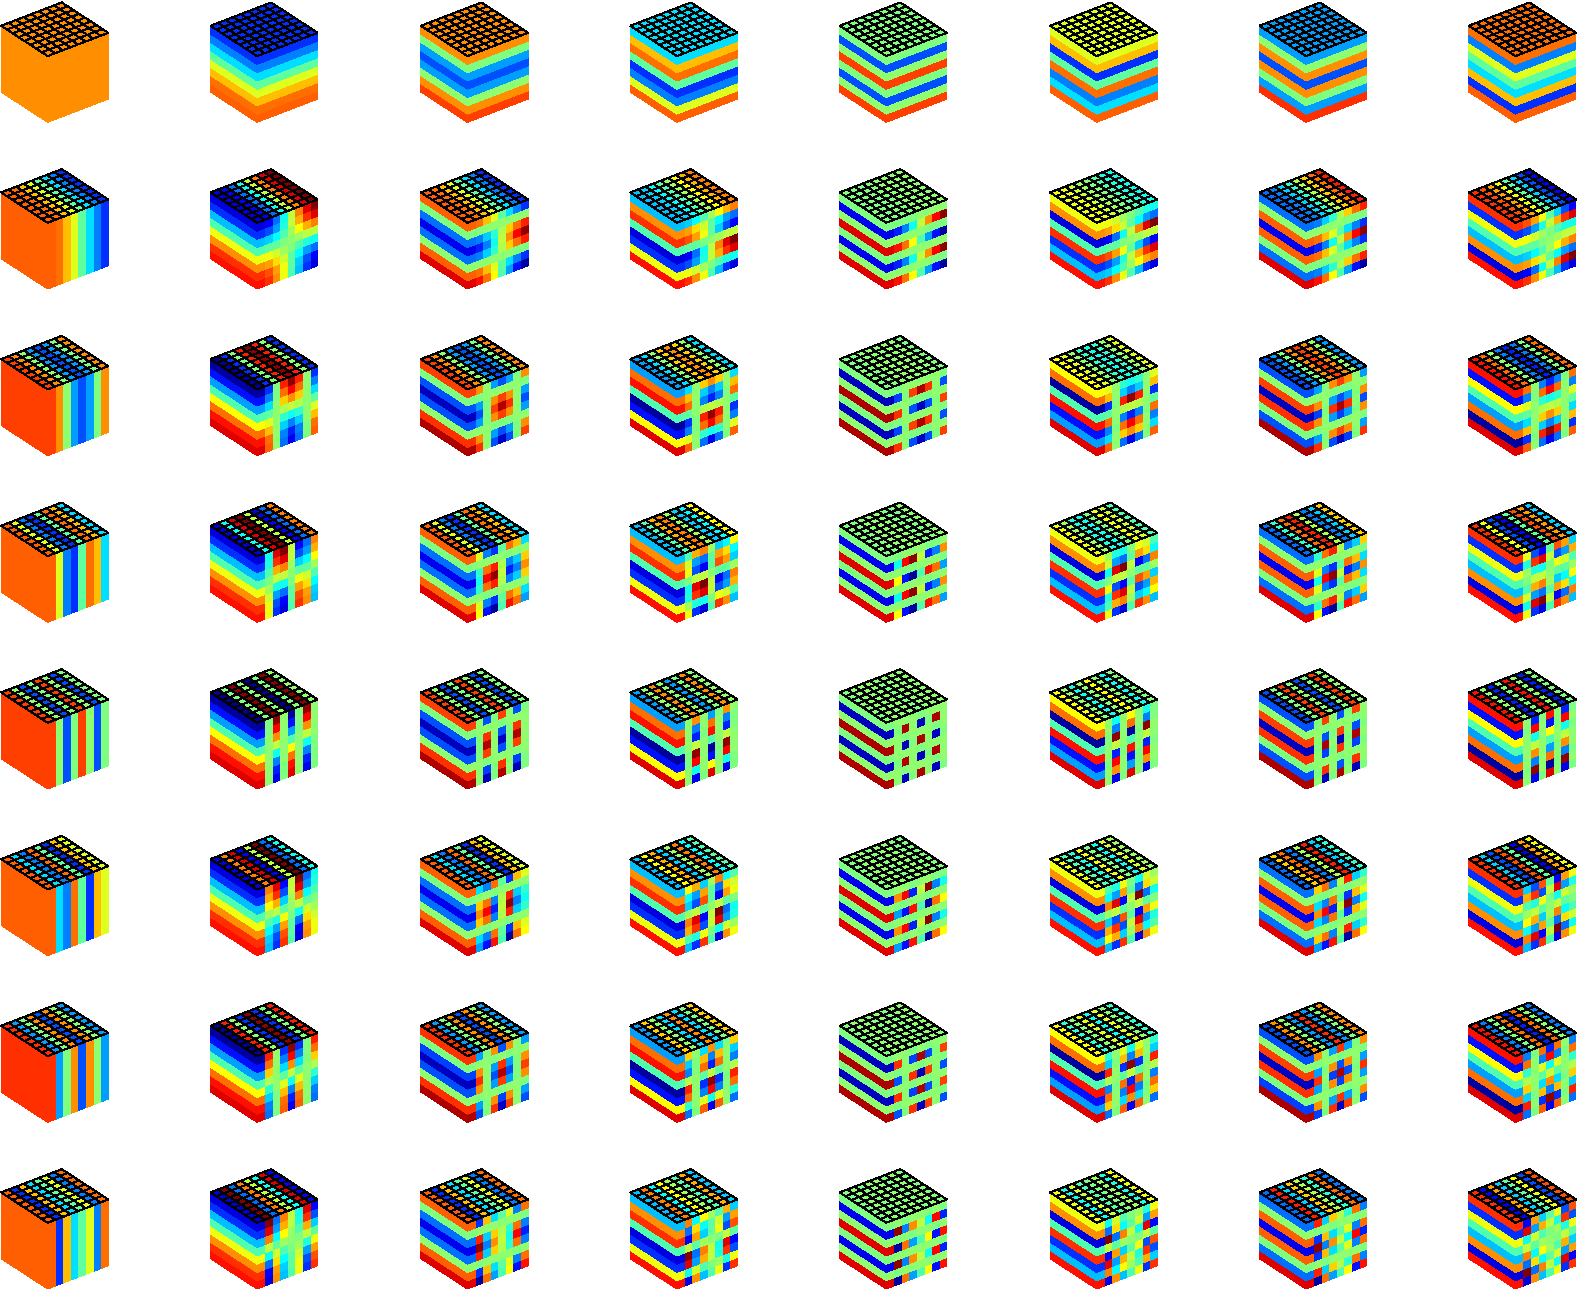
\includegraphics[width=0.5\textwidth]{Fig/t-atoms1}
   \label{fig:t-atoms1}}\\
   \subfloat[]{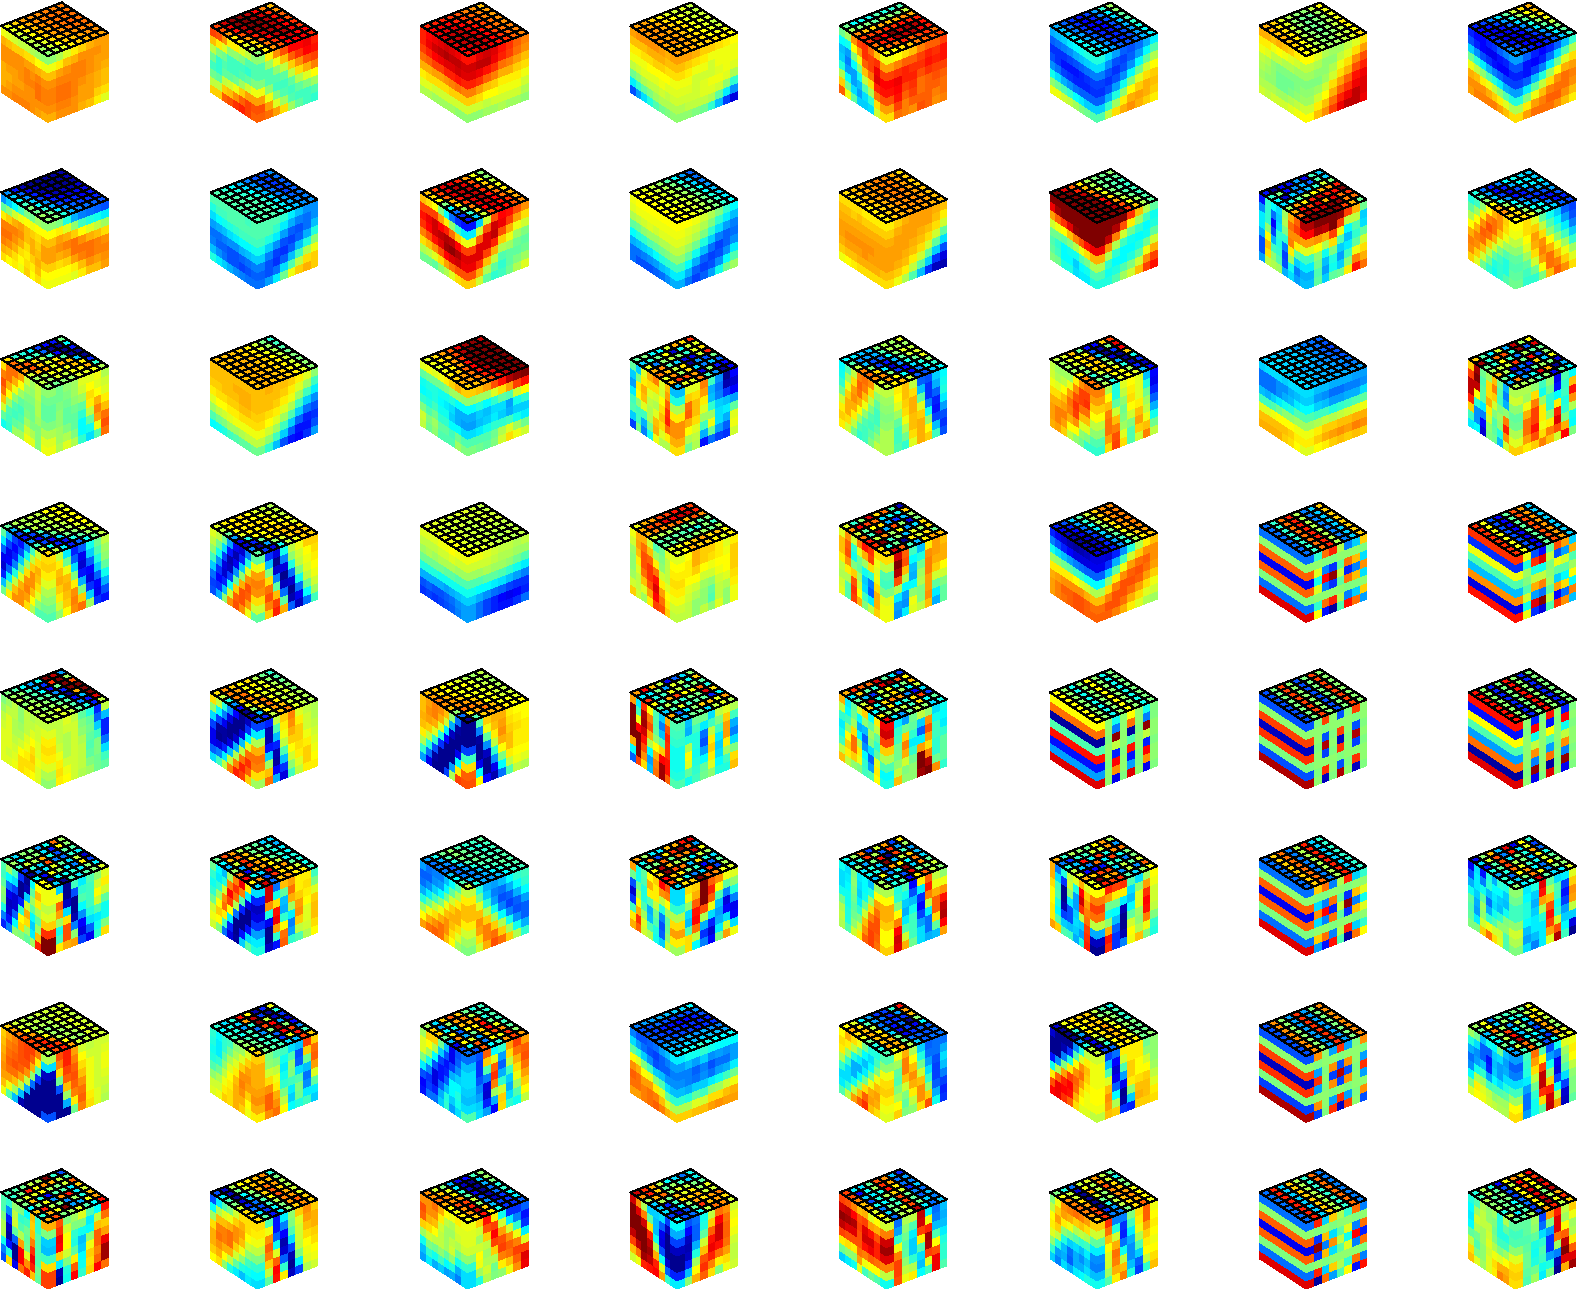
\includegraphics[width=0.5\textwidth]{Fig/t-atoms2}
   \label{fig:t-atoms2}}
\caption{Comparison between the initial atoms (a) and learned atoms (b). }
\label{fig:t-atoms1,t-atoms2}
\end{figure}

\begin{figure}[htb!]
\centering

   \subfloat[]{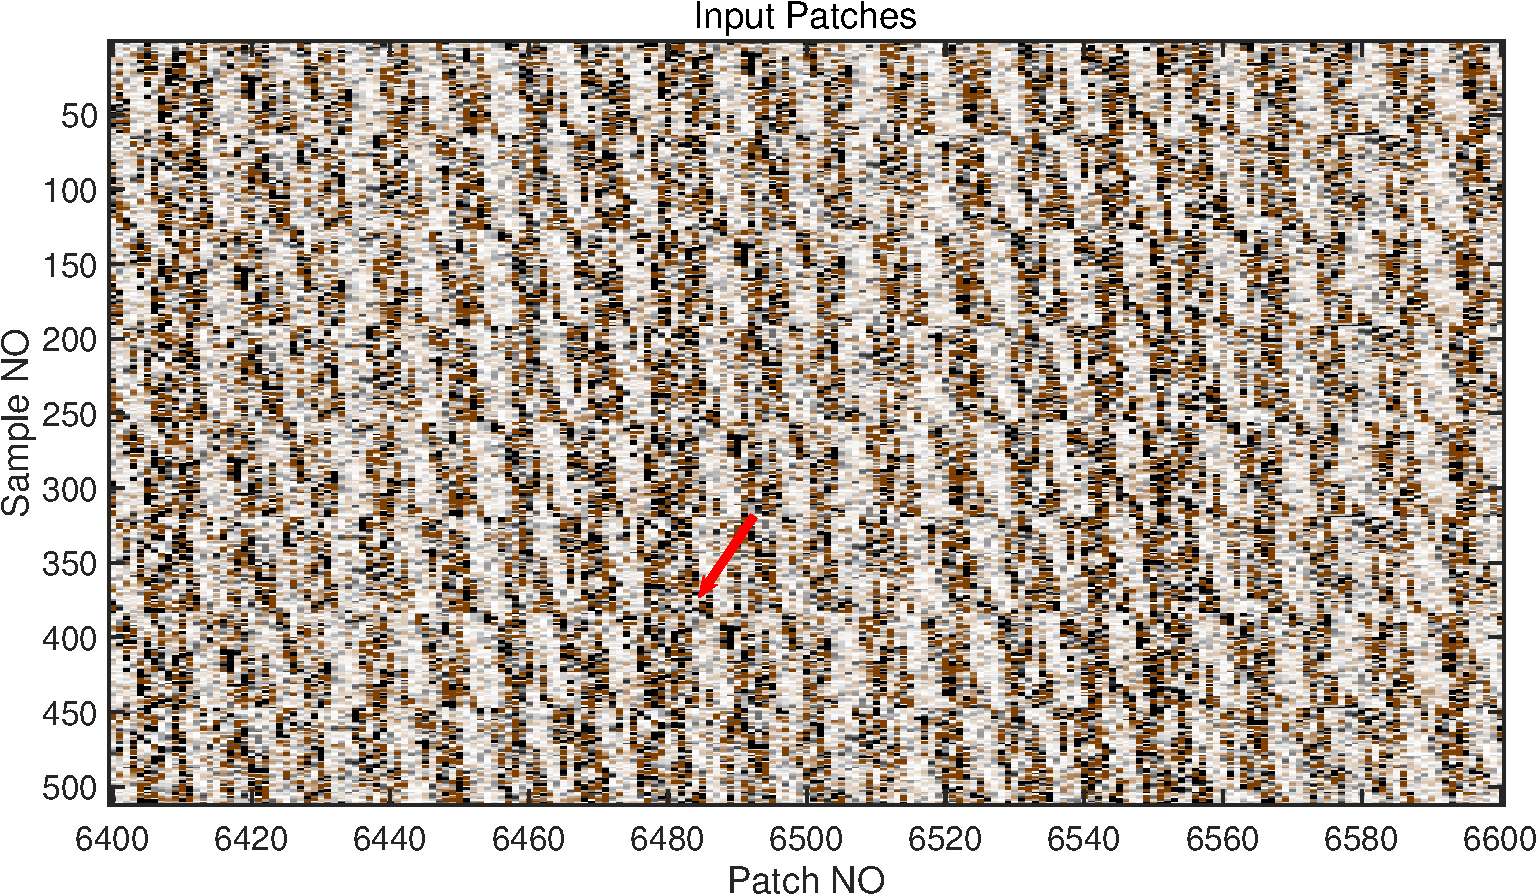
\includegraphics[width=0.7\textwidth]{Fig/t_XXn_z}
   \label{fig:t_XXn_z}}\\
   \subfloat[]{\includegraphics[width=0.7\textwidth]{Fig/t_Xn_z}
   \label{fig:t_Xn_z}}%\\
%   \subfloat[]{\includegraphics[width=0.45\textwidth]{Fig/t_Xnn}
%   \label{fig:t_Xnn}}
%   \subfloat[]{\includegraphics[width=0.45\textwidth]{Fig/t_Xnn_z}
%   \label{fig:t_Xnn_z}}
\caption{Comparison of different patches. \old{(a) Input patches created from the initial noise. (b) Zoomed patches from (a). (c) Output patches after dictionary learning and thresholding. (d) Zoomed patches from (b). \dlo{(e) Difference of patches between (a) and (c). (f) Zoomed patches from (e).} The zooming areas are highlighted by the red frame boxes. Note the clear retrieved signal patches.} \new{(a) Input patches created from the initial noise. (b) Output patches after dictionary learning and thresholding.}}
\label{fig:t_XXn_z,t_Xn_z}
\end{figure}
}


Finally, we test the performance of the proposed method on the TeapotDome 3D dataset ($900\times 75\times 150$ \wen{and sampling rate is 2 ms, and dominant frequency is about 40 Hz}), which is plotted in Figure \ref{fig:tea}. Figures \ref{fig:t-fxy}-\ref{fig:t-dl} plot the denoised data using the $f-x-y$ non-stationary predictive filtering (FXY) method \cite[]{wanghang2021geo}, the local orthogonalization method, and the proposed method, respectively. From the denoised data, it seems that all three methods obtain successful denoising performance. However, when compared in the removed noise cubes, the differences between different methods become clear. The FXY method causes significant damages to the useful signals, as pointed by the labeled arrows in Figure \ref{fig:t-fxy-n0}. The local orthogonalization method helps retrieve some leaked signals, and the signal energy in the noise cube becomes weaker, as pointed out by the arrow in Figure \ref{fig:t-ortho-n0}. However, the coherent signal energy is still visible in the noise cube in Figure \ref{fig:t-ortho-n0}.  The proposed DL method mitigates the signal leakage to a great extent and the coherent signal energy in the noise cube is almost negligible, as indicated by the arrows in Figure \ref{fig:t-dl-n0}. To better visualize the differences, we extract a constant-time slice from each noise cube in Figure \ref{fig:t-fxy-n0,t-ortho-n0,t-dl-n0} and show them in Figure \ref{fig:slice-fxy-0,slice-ortho-0,slice-dl-0,slice-fxy-z,slice-ortho-z,slice-dl-z}. Figures \ref{fig:slice-fxy-0}-\ref{fig:slice-dl-0} show the time slices in the original scale and Figures \ref{fig:slice-fxy-z}-\ref{fig:slice-dl-z} show the zoomed time slices from the pink frame boxes. From Figure \ref{fig:slice-fxy-0,slice-ortho-0,slice-dl-0,slice-fxy-z,slice-ortho-z,slice-dl-z}, it is very clear that the signal leakage becomes weaker and weaker from left to right. Figure \ref{fig:t-comp} shows a concatenated dataset showing a detailed comparison among initial result, initial noise, recovered leaked signals, new result, new noise (from left to right in the front panel).  It is clear that the dictionary learning process effectively retrieves those leaked signals without bringing back the incoherent noise, thus making the denoised reflection signals stronger. Figure \ref{fig:t-atoms1,t-atoms2} shows a comparison of the initial (a) and learned (b) dictionaries by plotting each dictionary atom as a 3D cube ($8\times 8 \times8$). It is clear that the dictionary learning process effectively extracts significant signal features from the data, which are crucial in retrieving the leaked signals in the 3D noise cube of a traditional method. Figure \ref{fig:t_XXn_z,t_Xn_z} plots a comparison of the input and output patches after the learning and coding the sparse dictionary. Figures \ref{fig:t_XXn_z} and \ref{fig:t_Xn_z}\dlo{, and \ref{fig:t_Xnn}} correspond to the input and output\dlo{, and difference} patches. \old{Figures \ref{fig:t_XXn_z} and \wen{\ref{fig:t_Xn_z}}\dlo{, and \ref{fig:t_XXn_z}} correspond to zoomed patches from the red frame boxes.} We can see that the proposed method can successfully retrieve those useful signals from very noise patches. While most noise patches are untouched, a significant amount of signal energy can be effectively detected and extracted. 


\section{Discussion}
In the local orthogonalization method, the main parameter is the smoothing radius. A larger smoothing radius can mitigate the retrieval of random noise but could fail in retrieving the small-scale leaked signals, while a smaller smoothing radius is able to retrieve the small-scale signal leakage but could retrieve more noise, causing significant residual noise in the denoised data. In the proposed DL method, the main controlling parameter is the percentage of largest coefficients to be preserved in the sparse coefficients matrix $\mathbf{M}$. Thus, the proposed method is nearly an automatic algorithm to retrieve the leaked signals. To investigate how the percentage affects the signal retrieving performance, we compare retrieved sections using different percentages in Figure \ref{fig:pp-re-p1-0,pp-re-p2-0,pp-re-p3-0,pp-re-p4-0}. Figures \ref{fig:pp-re-p1-0}-\ref{fig:pp-re-p4-0} correspond to $p=0.3\%$, $p=0.6\%$, $p=1\%$, and $p=2\%$, respectively. It is clear that while all percentage values help retrieve the key leaked signals, the retrieved noise becomes stronger when $p$ increases. In practical usage, the percentage should be a small value, e.g., $<2\%$, one may need to adjust several times to obtain the best performance depending on the user's preference. Note that the small-scale leaked signals may look quite similar to the noise, thus sometimes one may choose to retrieve more noise to ensure no leaked small-scale signals. Some other parameters, like the patch size, shifting size, and sparsity level $T$, may affect the performance but not significantly. For example, a larger patch size has a stronger anti-noise ability and tends to obtain smoother dictionary atoms due to better coherency of the signals in a larger window, but tends to lose the resolution to retrieve the small-scale signals. A smaller patch size is more capable of retrieving small-scale signals but tends to be more sensitive to noise. For all the examples in this paper, we use a square/cubic patch with the length of a single side as eight samples. Some studies have shown that the vertical patch size is optimally chosen as half of the dominant wavelength \cite[]{guoyin2018,wanghang2020}. Other parameters like the shifting size and sparsity level could also slightly affect the performance, but we all fix them to be the default values (e.g., the shift size is two samples, and the sparsity level $T=3$) for all the examples in this paper. 

The computational cost of the DL method is higher than the local orthogonalization method, even with the proposed fast dictionary learning scheme. For example, for the first field data example $1024\times 471$, the local orthogonalization method takes 2.03 s, and the proposed method takes 110.32 s. For the 3D Teapot Dome dataset, the proposed method takes less than an hour while the local orthogonalization method takes less than one minute. \wen{The comparison of running time during dictionary learning is listed in Table \ref{tbl:time} and compared with the KSVD algorithm. } The computation is carried out on a Mac Pro laptop with 2.5 GHz Intel Core i7 and 16 GB Ram. Although more expensive than the local orthogonalization method, the proposed method is still affordable. The dictionary learning step has been significantly accelerated by the SGK method due to the special sparse coding step and the SVD-free implementation. According to our experience and some published results, the SGK method can be 6-12 times faster than the traditional KSVD method. Generally speaking, the proposed method is affordable in industrial-scale applications. 

\begin{table}[h]
\caption{Running time comparison during dictionary learning.}
\begin{center}
    \begin{tabular}{|c|c|c|c|c|c|} 
  \hline    & Synthetic & 2D field  & 3D field \\ 
  \hline SGK (s) & \new{3.1}  & \new{30.1}  & \new{825.5}\\
  \hline KSVD(s) & \new{26.5} & \new{313.5} & \new{6403.3} \\
      \hline
   \end{tabular} 
\end{center}
\label{tbl:time}
\end{table}

\AtEndDocument{
\begin{figure}[htb!]
\centering
   \subfloat[]{\includegraphics[width=0.45\textwidth]{real2d/Fig/pp-re-p1-0}
   \label{fig:pp-re-p1-0}}
   \subfloat[]{\includegraphics[width=0.45\textwidth]{real2d/Fig/pp-re-p2-0}
   \label{fig:pp-re-p2-0}}\\
   \subfloat[]{\includegraphics[width=0.45\textwidth]{real2d/Fig/pp-re-p3-0}
   \label{fig:pp-re-p3-0}}
   \subfloat[]{\includegraphics[width=0.45\textwidth]{real2d/Fig/pp-re-p4-0}
   \label{fig:pp-re-p4-0}}\\
\caption{Effect of percentage values. (a) Retrieved section using $p=0.3\%$. (b) Retrieved section using $p=0.6\%$. (c) Retrieved section using $p=1\%$. (d) Retrieved section using $p=2\%$.  }
\label{fig:pp-re-p1-0,pp-re-p2-0,pp-re-p3-0,pp-re-p4-0}
\end{figure}
}

\section{Conclusions}
The local signal-and-noise orthogonalization method is effective in retrieving the leaked seismic signals from the removed noise profile. However, due to the strong non-stationarity of seismic data, the smoothing radius parameter of the local orthogonalization method is not easy to adjust, which makes it difficult to retrieve the useful signals without bringing back too much random noise. To retrieve the signals in a more adaptive way, we need to either apply a local orthogonalization method in a non-stationary way where the non-stationary input parameter is difficult to choose or apply a new patch-based method that is less dependent on the manually chosen parameter. The proposed dictionary learning method retrieves the leaked useful signals in a patch-based way. The learned dictionary from the initially denoised data can effectively capture the features of seismic signals. Because of a diverse range of dictionary atoms and the sparse coding process based on the orthogonal matching pursuit method, it is easy to retrieve the leaked signals adaptively. The synthetic and field data examples both show that the proposed method performs successfully in practical situations. 

\section{DATA AND MATERIALS AVAILABILITY}
Data associated with this research are available and can be obtained by contacting the corresponding author.


\bibliographystyle{seg}
\bibliography{dl}



